\mainmatter
\chapter{Introduzione} \label{chapter:intro}
L'obiettivo di tale relazione è quello di esporre quanto è stato realizzato durante il periodo di stage, svoltosi presso l'azienda Sync Lab srl, operante nel settore dell'IT Consultant \& Service. Il tirocinio, della durata di 3 mesi, ha coinvolto attività di formazione sui framework Spring\aref{appendix:spring}, Hibernate\aref{appendix:hibernate} e Angular\aref{appendix:angular} e l'attuazione di quanto appreso mediante progettazione e sviluppo di un'applicazione web, oggetto di questa tesi.

\section{TEMPO}
Il software progettato è un prodotto gestionale, sviluppato per l'azienda presso cui si è svolta l'attività, il cui compito primario è quello di permettere la gestione della rendicontazione dell'orario di lavoro giornaliero del singolo dipendente, in relazione ai clienti ad esso associati. Lo scopo principale è stato, quindi, quello di sviluppare un sistema in grado di gestire un discreto numero di utenze, una per ogni dipendente, e che, a seconda del livello gerarchico in azienda, fornisca una serie di funzionalità, tra cui permettere l'inserimento dell'attività svolta giornalmente con il relativo numero di ore lavorate. Inoltre, il sistema deve essere in grado di memorizzare l'anagrafica dei dipendenti e dei clienti per tenere traccia degli eventuali progetti attivi e conclusi, e il numero di risorse che vi sono allocate. In particolare ogni volta che una risorsa viene allocata presso un cliente, a questa viene assegnato un codice univoco, il quale mette in relazione, oltre a cliente e risorsa, anche l'attività svolta e il progetto su cui il dipendente viene assegnato.

L'applicazione in questione è stata denominata TEMPO, una sorta di acronimo costituito da una combinazione di alcune tra le prime lettere delle parole \textit{Employees' Timesheet Portal}.

\section{Processo software utilizzato}
Il processo software adottato per la creazione di tale prototipo è UP (\textit{Unified Process}), ossia un framework agile per la gestione del ciclo di sviluppo del software, iterativo ed incrementale, e concepito per gestire progetti e prodotti software. A partire quindi dalla specifica fornita, sono state effettuate in alternanza, delle fasi di analisi dei requisiti, progettazione, implementazione e test. In questo modo è stato possibile garantire la realizzazione di un prodotto in grado di soddisfare le esigenze richieste e la gestione di eventuali casi eccezionali o di errore. Tuttavia, date le dimensioni discrete del software da progettare, sarebbe stato possibile adottare un processo a cascata, ormai obsoleto in ogni contesto di sviluppo di medie o grandi dimensioni. Si è comunque deciso di adottare un processo software \textit{agile}, in quanto propedeutico per il mondo lavorativo, ma soprattutto perché più efficiente e riduce al minimo la probabilità di fallimento.

\section{Unified Modeling Language}
Per quanto riguarda la progettazione, si è fatto uso del linguaggio UML (\textit{Unified Modeling Language}), ossia un linguaggio di modellazione e di specifica molto utile quando si utilizza il paradigma di programmazione orientata agli oggetti. Esso permette, tramite l’utilizzo di modelli visuali, di analizzare, descrivere, specificare e documentare un sistema software, anche complesso. In particolare sono stati utilizzati i seguenti diagrammi:
\begin{itemize}
    \item Diagramma dei casi d'uso, utile per la rappresentazione visuale e sintetica dei casi d'uso sviluppati.
    \item Diagramma di sequenza, sostanzialmente legato al diagramma dei casi d'uso ed utilizzato per definire la serie di azioni compiute dall'utente e dal sistema quando viene richiesto un determinato servizio, andando a mostrare le interazioni tra i due e gli altri eventuali attori coinvolti.
    \item Diagramma delle classi, forse quello più importante tra tutti e che rappresenta la struttura dell'intero progetto. Da tale diagramma si andranno poi a definire le classi Java, e le relazioni fra di esse, che andranno a comporre l'applicazione.
    \item Diagramma di attività, utilizzato per mostrare i vari passi compiuti nelle varie attività che vengono eseguite per espletare una determinata funzione o servizio previsti dal sistema.
\end{itemize}

\section{Pattern MVC e REST API}
Un ulteriore obiettivo è stato quello di assicurare le principali caratteristiche che un buon software deve possedere, tra cui scalabilità, sicurezza e manutenibilità. Per tale ragione si è pensato ad un'architettura mirata a garantire l'indipendenza fra i vari componenti, utilizzando il pattern MVC (\textit{Model View Controller}) unito ad un web service di tipo REST.

\subsection{Model View Controller}
Model View Controller (comunemente chiamato MVC) è un pattern di progettazione che definisce una struttura del codice dell'applicazione suddivisa in tre componenti differenti, ognuna indipendente dall'altra e con un compito preciso:
\begin{itemize}
    \item \textit{Model}: è responsabile della gestione dei dati dell'applicazione e dunque fornisce i metodi di accesso ad essi;
    \item \textit{View}: si occupa di visualizzare i dati all’utente e di gestire l’interazione fra quest’ultimo e l’infrastruttura sottostante;
    \item \textit{Controller}: riceve i comandi dell’utente attraverso la View e reagisce eseguendo delle operazioni che possono interessare il Model e che portano, generalmente, ad un cambiamento di stato della View.
\end{itemize}

\begin{figure}[H]
	\centering
	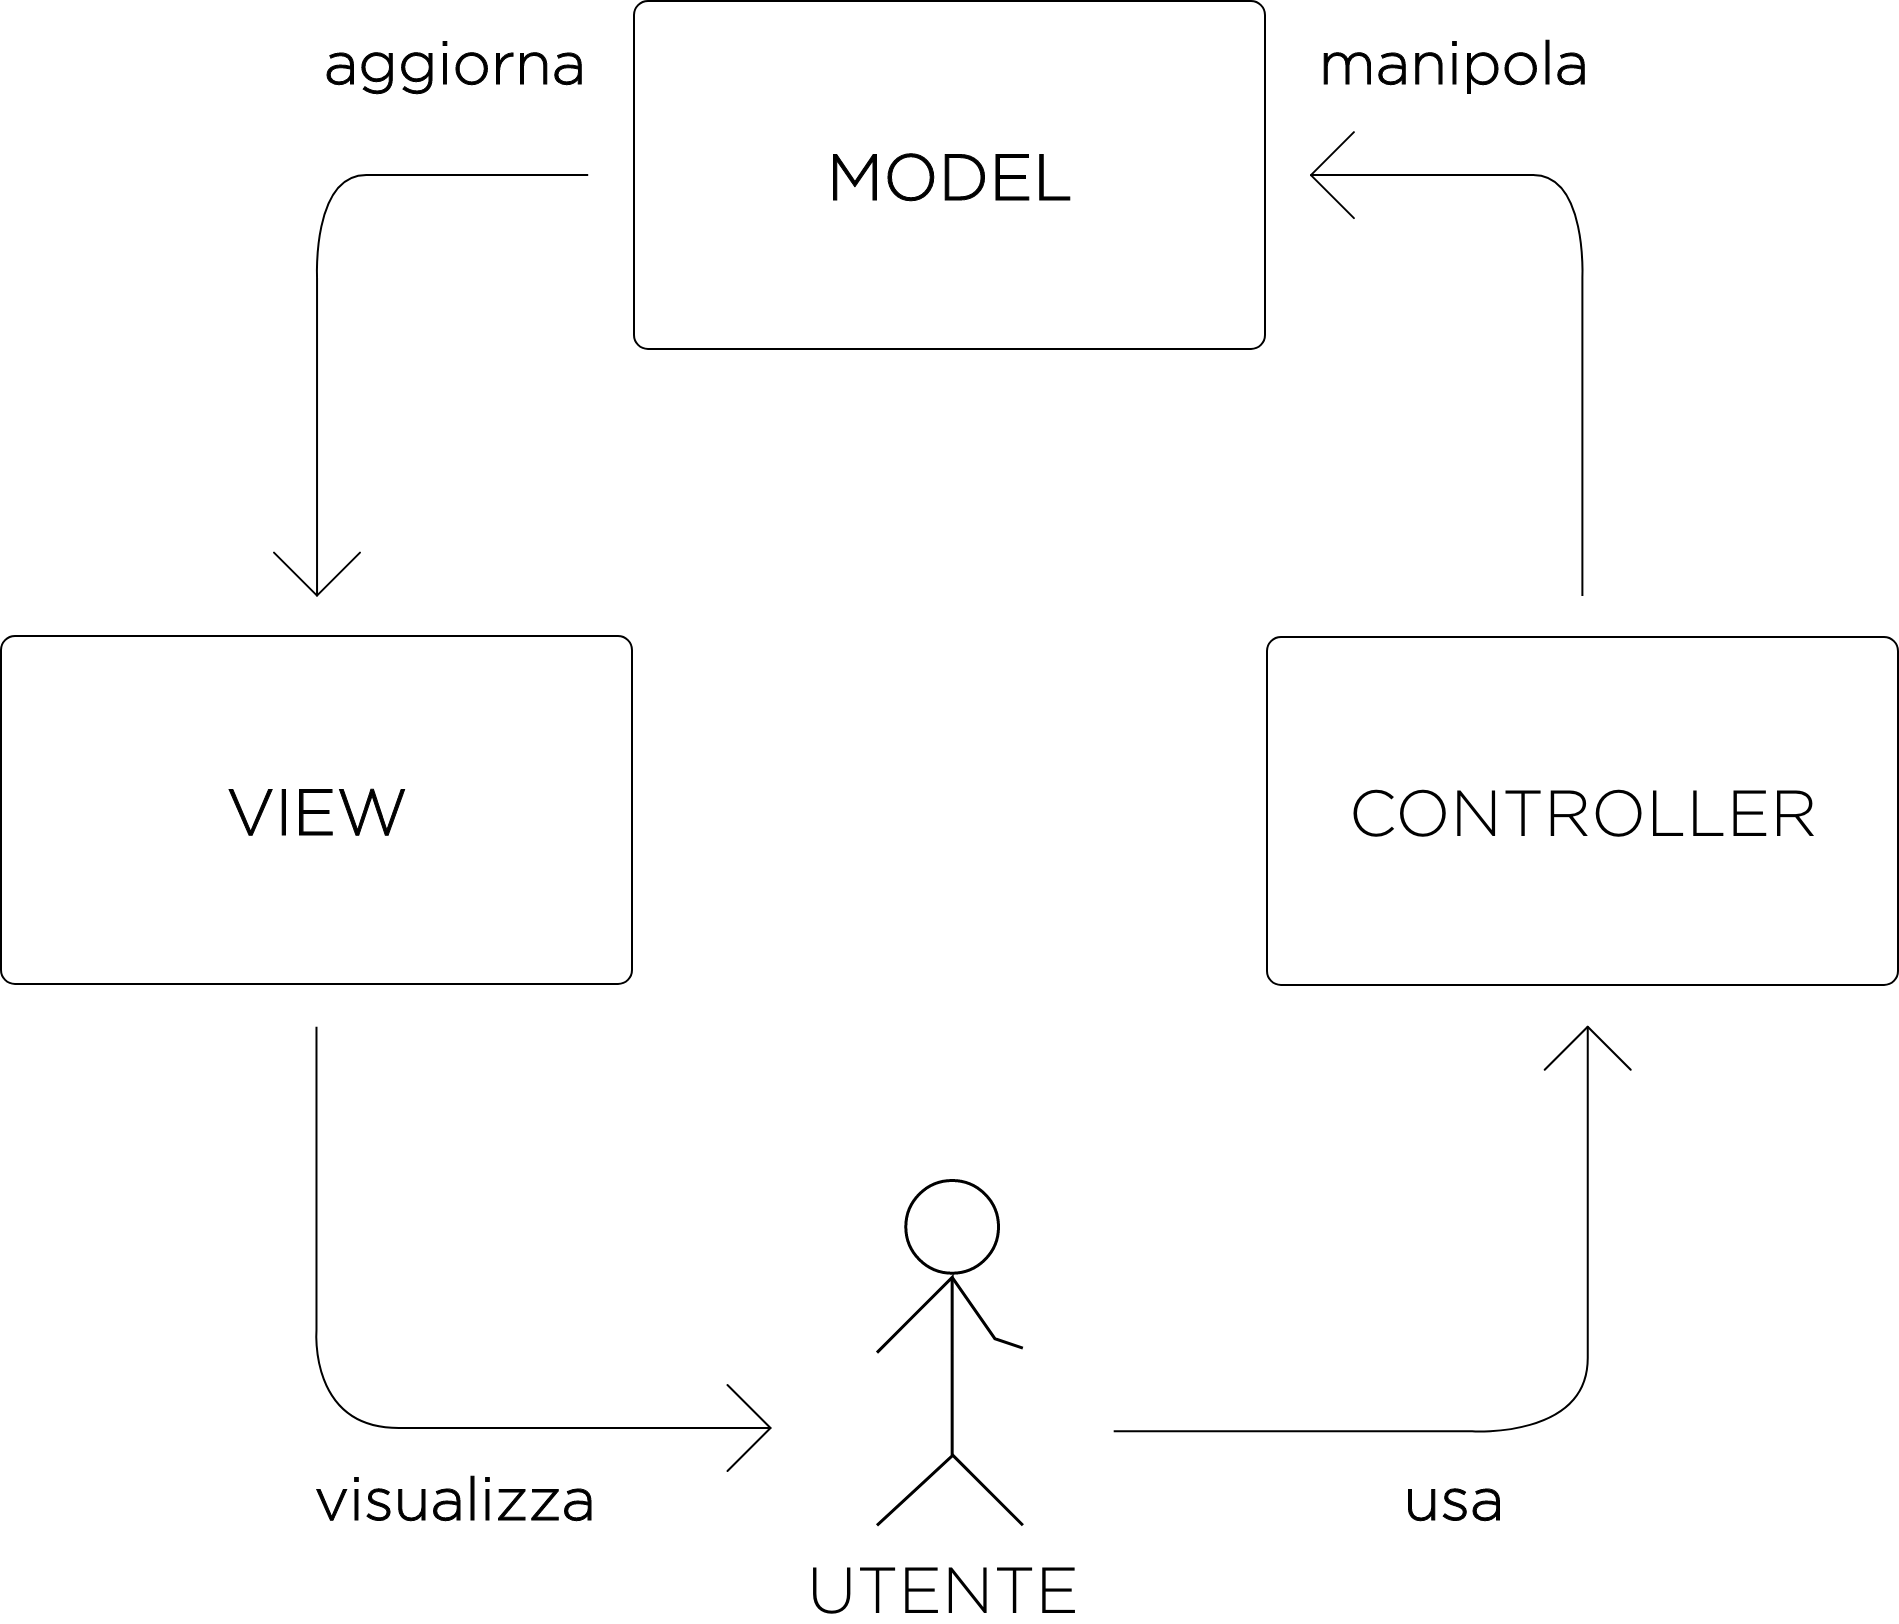
\includegraphics[width=.65\linewidth]{mvc.png}
	\caption{Schema di alto livello del pattern MVC.}
	\label{fig:mvc}
\end{figure}

\noindent
L'utilizzo di tale pattern ha il vantaggio principale di avere un codice comprensibile, riusabile e soprattutto mantenibile, in quanto vi è una separazione completa dei compiti da svolgere. Inoltre, grazie all'indipendenza tra i vari componenti si ha la possibilità di creare viste e controller diversi, utilizzando lo stesso modello di accesso ai dati e dunque, come già accennato, riutilizzando parte del codice esistente. Nel caso in cui si dovesse verificare un cambio al tipo di database, basterà apportare modifiche al modello, adattandolo alle esigenze e dunque senza dover cambiare il codice delle viste e dei controller.

\subsection{REST}
Quando si progetta un'applicazione web, un aspetto importante da considerare è sicuramente la fruibilità dei servizi che questa fornisce attraverso la rete. REST (\textit{REpresentational State Transfer}) è uno dei principi architetturali per la progettazione di un sistema \textit{network-based} e sostanzialmente offre un insieme di linee guida che si possono riassumere in 4 principi:
\begin{itemize}
    \item \textbf{Identificazione delle risorse}: ogni risorsa deve essere identificata univocamente ed essendo in ambiente web è naturale farlo mediante URI (\textit{Uniform Resource Identifier}).
    \item \textbf{Utilizzo esplicito dei metodi HTTP}: GET, POST, PUT e DELETE, rispettivamente per l'accesso, la creazione, la modifica e l'eliminazione di una risorsa e i quali si andranno a mappare alle operazioni CRUD (Create, Read, Update e Delete).
    \item \textbf{Risorse autodescrittive e collegate fra loro}: le risorse sono separate dalla rappresentazione restituita al client, il quale si preoccuperà lui stesso di definire nella richiesta HTTP il tipo di formato da restituire; ogni risorsa deve inoltre garantire i collegamenti a risorse correlate.
    \item \textbf{Comunicazione senza stato}: tale caratteristica fa parte del protocollo HTTP, difatti ciascuna richiesta non ha alcuna relazione con quelle precedenti e successive.
\end{itemize}

\noindent
Dunque per la creazione di un sistema RESTful è sufficiente che lato server venga implementato un servizio con le caratteristiche appena descritte. Mentre, lato client occorre un sistema in grado di effettuare richieste mediante protocollo HTTP, a delle URI che identificano le risorse, e in tali richieste si andrà a specificare un tipo di formato da ricevere che il client stesso sarà in grado di interpretare.

% removes the blank page after the end of the chapter
\let\cleardoublepage\clearpage
